\documentclass[11pt]{article}

\usepackage[margin=0.72in]{geometry}
\usepackage{booktabs}
\usepackage{tabularx}
\usepackage{newpxtext}
\usepackage{longtable}
\usepackage{array}
\usepackage{xcolor}
\usepackage{hyperref}
\usepackage{enumitem}
\usepackage{listings}
\usepackage{caption}
\usepackage{tcolorbox}
\usepackage{fontawesome}
\usepackage{tikz}
\usepackage{seqsplit}
\usetikzlibrary{positioning, arrows.meta, calc, shapes.geometric, fit, backgrounds}

\tcbuselibrary{skins,breakable}

\definecolor{tipblue}{HTML}{2D6CDF}
\definecolor{tipbg}{HTML}{EAF1FB}
\definecolor{warnorange}{HTML}{D17B00}
\definecolor{warnbg}{HTML}{FFF4E0}
\definecolor{codegray}{HTML}{F5F5F5}
\definecolor{accent}{HTML}{0B5394}

\hypersetup{
  colorlinks=true,
  linkcolor=accent,
  urlcolor=accent,
  citecolor=accent,
  pdftitle={ASMx Data Documentation},
  pdfauthor={ASMx contributors}
}

\lstset{
  basicstyle=\ttfamily\footnotesize,
  backgroundcolor=\color{codegray},
  breaklines=true,
  frame=single,
  framesep=4pt,
  framerule=0pt,
  xleftmargin=6pt,
  showstringspaces=false,
  columns=fullflexible,
  keepspaces=true
}

\newcolumntype{L}[1]{>{\raggedright\arraybackslash}p{#1}}
\newcommand{\code}[1]{\texttt{#1}}
\newcommand{\nan}{\code{NaN}}
\newcommand{\filename}[1]{\textcolor{accent}{\code{#1}}}

% Allow TeX to stretch interword spaces a little before giving up — keeps
% long \texttt{...} paths from causing minor overfull boxes.
\setlength{\emergencystretch}{3em}

\newtcolorbox{tipbox}{
  enhanced, breakable,
  colback=tipbg, colframe=tipblue, boxrule=0.4pt,
  arc=2pt, left=8pt, right=8pt, top=4pt, bottom=4pt,
  title={\textbf{\faInfoCircle\ \ Tip}}, fonttitle=\small,
  coltitle=tipblue, colbacktitle=tipbg,
  attach boxed title to top left={xshift=8pt, yshift*=-\tcboxedtitleheight/2},
  boxed title style={colback=tipbg, colframe=tipbg, boxrule=0pt}
}
\newtcolorbox{warnbox}{
  enhanced, breakable,
  colback=warnbg, colframe=warnorange, boxrule=0.4pt,
  arc=2pt, left=8pt, right=8pt, top=4pt, bottom=4pt,
  title={\textbf{\faExclamationTriangle\ \ Heads-up}}, fonttitle=\small,
  coltitle=warnorange, colbacktitle=warnbg,
  attach boxed title to top left={xshift=8pt, yshift*=-\tcboxedtitleheight/2},
  boxed title style={colback=warnbg, colframe=warnbg, boxrule=0pt}
}

\title{\vspace{-1.5em}\textbf{\Huge ASMx Data Documentation}\\[0.6em]
\large A documentation to the datasets associated with the
\emph{Calibrating Adaptive Smoothing Methods for Freeway Traffic
Reconstruction} repository}
\author{}
\date{}

\begin{document}
\maketitle
\vspace{-3em}

\begin{center}
\begin{tcolorbox}[width=0.92\textwidth, colback=tipbg, colframe=tipblue,
  boxrule=0.4pt, arc=3pt, halign=left]
\textbf{What this document is.} A user-oriented guide to every dataset in
\code{data/} of the ASMx repository. For each file it explains contents, the
meaning of columns or array axes, units, and how to load the data in Python.
Dataset descriptions follow Section~3.1 of the accompanying paper \textit{Calibrating Adaptive Smoothing Methods for Freeway Traffic Reconstruction}; the paper contains further methodological and experimental details. This guide aims to clarify the data at all stages (raw query records, processed raw data, preprocessed datasets, etc.).
\end{tcolorbox}
\end{center}

\tableofcontents
\bigskip

%---------------------------------------------------------------
\section{Quick start}

\subsection*{Just want to load the calibration data?}

\begin{lstlisting}[language=Python]
import numpy as np

# Sparse RDS speed observations (the model input \tilde X in the paper)
rds = np.load('data/processed_data/rds/lane1/2024-07-09.npy')
# MOTION ground-truth speed field (the calibration target X-hat)
gt  = np.load('data/processed_data/motion/lane1/2024-07-09.npy')

print(rds.shape, gt.shape)   # (200, 3600) (200, 3600)
print(rds.dtype)             # float32
# Row index = space cell (200 cells from MM 58.7 to MM 62.7, dx = 0.02 mi)
# Col index = time cell (3600 cells from 06:00 to 10:00, dt = 4 s)
# Values    = speed in mph (multiply by 1.60934 for km/h, as the paper does)
\end{lstlisting}

\subsection*{The three-stage data pipeline at a glance}

The two measurement modalities (RDS and MOTION) flow through the same three
stages and meet on the same processed grid in Stage~3. The corridor-scale
variant under \code{corridor\_data/} mirrors Stage~3 for the wider
27.36~km window.

\begin{figure}[h]
\centering
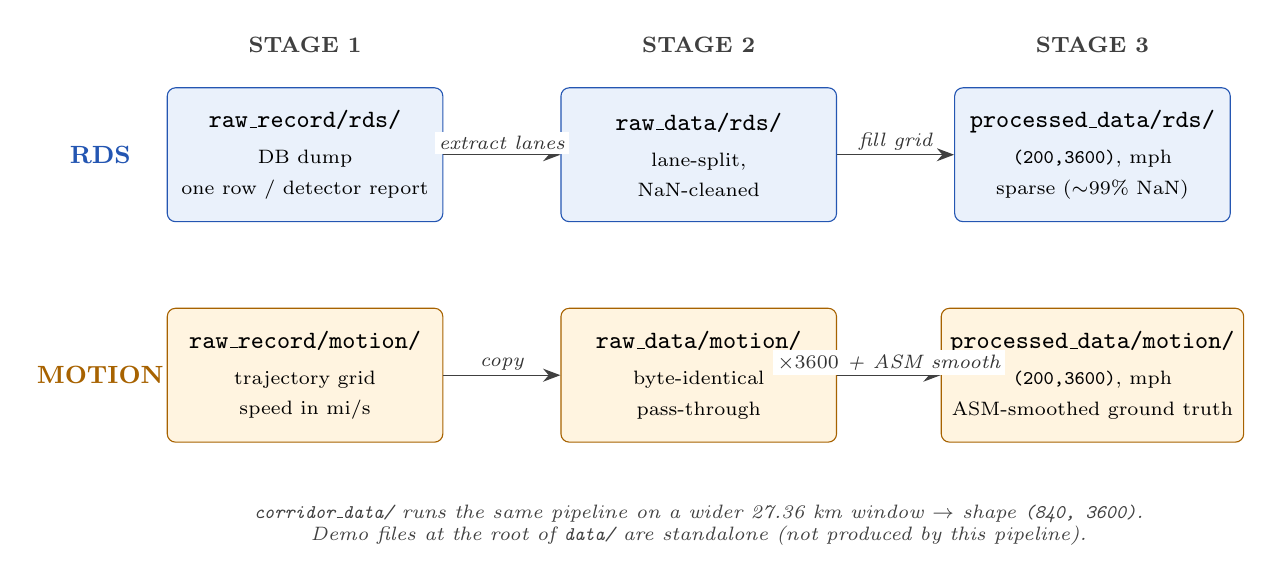
\begin{tikzpicture}[
  >={Stealth[length=2.2mm]},
  font=\small,
  stage/.style={
    draw, rounded corners=3pt,
    minimum width=3.5cm, minimum height=1.7cm,
    align=center, line width=0.4pt
  },
  rds/.style={stage, fill=tipbg, draw=tipblue!80!black},
  motion/.style={stage, fill=warnbg, draw=warnorange!80!black},
  output/.style={stage, fill=gray!8, draw=gray!60!black,
    minimum width=3.5cm, minimum height=1.7cm},
  modlabel/.style={font=\bfseries\small},
  stagelabel/.style={font=\bfseries\footnotesize, gray!50!black},
  arr/.style={->, line width=0.5pt, gray!50!black},
  arrlabel/.style={font=\scriptsize\itshape, gray!40!black, fill=white,
    inner sep=1.5pt, midway}
]

% Stage column headers
\node[stagelabel] at (0, 2.4)  {STAGE 1};
\node[stagelabel] at (5.0, 2.4) {STAGE 2};
\node[stagelabel] at (10.0, 2.4) {STAGE 3};

% RDS row
\node[modlabel, tipblue!80!black] at (-2.6, 1.0) {RDS};
\node[rds] (r1) at (0, 1.0)
  {\code{raw\_record/rds/}\\[2pt]
   \scriptsize DB dump\\\scriptsize one row / detector report};
\node[rds] (r2) at (5.0, 1.0)
  {\code{raw\_data/rds/}\\[2pt]
   \scriptsize lane-split,\\\scriptsize NaN-cleaned};
\node[rds] (r3) at (10.0, 1.0)
  {\code{processed\_data/rds/}\\[2pt]
   \scriptsize \code{(200,3600)}, mph\\\scriptsize sparse ($\sim$99\% NaN)};

% MOTION row
\node[modlabel, warnorange!80!black] at (-2.6, -1.8) {MOTION};
\node[motion] (m1) at (0, -1.8)
  {\code{raw\_record/motion/}\\[2pt]
   \scriptsize trajectory grid\\\scriptsize speed in mi/s};
\node[motion] (m2) at (5.0, -1.8)
  {\code{raw\_data/motion/}\\[2pt]
   \scriptsize byte-identical\\\scriptsize pass-through};
\node[motion] (m3) at (10.0, -1.8)
  {\code{processed\_data/motion/}\\[2pt]
   \scriptsize \code{(200,3600)}, mph\\\scriptsize ASM-smoothed ground truth};

% Arrows + labels
\draw[arr] (r1) -- node[arrlabel, above]{extract lanes} (r2);
\draw[arr] (r2) -- node[arrlabel, above]{fill grid} (r3);
\draw[arr] (m1) -- node[arrlabel, above]{copy} (m2);
\draw[arr] (m2) -- node[arrlabel, above]{$\times 3600$ + ASM smooth} (m3);

% Note about corridor + demo
\node[font=\scriptsize\itshape, gray!50!black, align=center]
  at (5.0, -3.7)
  {\code{corridor\_data/} runs the same pipeline on a wider 27.36~km window
   $\to$ shape \code{(840, 3600)}.\\
   Demo files at the root of \code{data/} are standalone (not produced by
   this pipeline).};

\end{tikzpicture}
\caption{The three-stage data pipeline. The RDS track produces the sparse
model input $\tilde{\mathcal{X}}$; the MOTION track produces the dense
ground truth $\hat{\mathcal{X}}$. Both end up on the same
\code{(200,3600)} mph grid, so they can be overlaid without any rescaling.}
\label{fig:pipeline-diagram}
\end{figure}

\subsection*{What file do I need?}

\begin{tabularx}{\textwidth}{L{3.2cm} L{4.4cm} X}
\toprule
\textbf{Stage} & \textbf{If you want to\dots} & \textbf{Open\dots} \\
\midrule
Stage 1 \newline (\code{raw\_record/})
  & Inspect raw detector readings before any cleaning
  & \filename{raw\_record/rds/\{date\}.csv} (one row per detector report). \\
\addlinespace
Stage 1 \newline (\code{raw\_record/})
  & Re-run the preprocessing yourself end-to-end
  & Start from \filename{raw\_record/}, run scripts in \code{preprocessing/}. \\
\addlinespace
Stage 2 \newline (\code{raw\_data/})
  & Inspect lane-split, time-snapped detector readings
  & \filename{raw\_data/rds/\{date\}.csv} (one row per (MM, 30~s bin)). \\
\addlinespace
Stage 3 \newline (\code{processed\_data/})
  & Reproduce the lane-1 calibration in Sec.~3.2 (July~9, 2024)
  & \filename{processed\_data/rds/lane1/2024-07-09.npy} \newline (model input) \newline
    \filename{processed\_data/motion/lane1/2024-07-09.npy} \newline (ground truth). \\
\addlinespace
Stage 3 \newline (\code{processed\_data/})
  & Run the cross-validation in Sec.~3.4
  & Both \code{processed\_data/} trees, all five dates
    (\code{2024-07-08} \dots \code{2024-07-12}), all four lanes. \\
\addlinespace
Corridor \newline (\code{corridor\_data/})
  & Reproduce the corridor-scale reconstruction in Fig.~13
  & \filename{corridor\_data/rds/lane1/2024-07-09.npy} \newline (840$\times$3600). \\
\addlinespace
Demo \newline (root of \code{data/})
  & Reproduce the I-95 use case in Fig.~14
  & \filename{I95speed.npy} (750$\times$4088). \\
\bottomrule
\end{tabularx}

\subsection*{Repository layout at a glance}

\begin{lstlisting}[basicstyle=\ttfamily\small,frame=none,backgroundcolor=\color{white}]
data/
|-- raw_record/        Stage 1: raw database dumps (one row per detector report)
|   |-- rds/{date}.csv
|   `-- motion/{date}/lane_{1..4}_speed_matrix.csv
|-- raw_data/          Stage 2: lane-split, time-snapped, NaN-cleaned CSVs
|   |-- rds/{date}.csv
|   `-- motion/{date}/lane_{1..4}_speed_matrix.csv
|-- processed_data/    Stage 3: regular (space, time) matrices, float32 .npy
|   |-- rds/lane{1..4}/{date}.npy        -> shape (200, 3600), sparse
|   `-- motion/lane{1..4}/{date}.npy     -> shape (200, 3600), dense ground truth
|-- corridor_data/     Same pipeline, but for the full 27.36 km SMART Corridor
|   `-- rds/{date}.csv  +  rds/lane{1..4}/{date}.npy  (shape (840, 3600))
|-- 2023-10-26.csv     Demo files, see Section 7
|-- 2025-04-09.csv
|-- I95speed.npy
|-- speed.npy
|-- asm_arxiv.pdf      The companion paper
`-- README.tex/.pdf    This document
\end{lstlisting}

%---------------------------------------------------------------
\section{What is in this dataset?}

\textbf{Site.} I-24 westbound near Nashville, TN. The primary study area is
the I-24~MOTION testbed (6.76~km of instrumented roadway, MM~58.7--62.7);
demonstration files also cover the wider I-24~SMART~Corridor (27.36~km,
MM~53.3--70.1) and an I-95 northbound segment in Virginia (MM~115--130).

\textbf{When.} Five consecutive weekdays, 2024-07-08 through 2024-07-12 (Mon
through Fri), 06:00--10:00 local time (America/Chicago). The canonical date
list is \filename{../dates.csv}.

\textbf{Two measurement modalities} are propagated through three pipeline
stages:

\begin{itemize}[leftmargin=*]
  \item \textbf{RDS} (Radar Detector System). Fixed-location Wavetronix
    SmartSensor HD radar sensors at $\approx$483~m ($\approx$0.3~mi) spacing,
    reporting 30-second aggregated speed, occupancy, and volume. This is the
    \emph{sparse model input} $\tilde{\mathcal{X}}$ in the paper.
  \item \textbf{MOTION}. Vehicle-trajectory--derived speed field from the
    I-24~MOTION testbed, computed per Edie's definition at 4-second temporal
    and 32-meter ($\approx$0.02~mi) spatial resolution using the parallelogram
    method. This is the \emph{dense ground truth} $\hat{\mathcal{X}}$.
\end{itemize}

\begin{tipbox}
The two modalities are co-registered onto the same processed grid (shape
\code{(200, 3600)}, $\Delta x = 0.02$~mi, $\Delta t = 4$~s, units of mph). You
can overlay them directly without any rescaling.
\end{tipbox}

\subsection{Conventions used everywhere}

\begin{tabularx}{\textwidth}{l X}
\toprule
\textbf{Item} & \textbf{Value} \\
\midrule
Spatial domain (calibration)    & Mile markers 58.7 $\to$ 62.7 (4 miles, westbound) \\
Spatial domain (corridor demo)  & Mile markers 53.3 $\to$ 70.1 (I-24 SMART Corridor) \\
Time zone                       & America/Chicago (UTC$-$05:00 in summer) \\
Time-of-day window              & 06:00--10:00 local \\
Dates                           & 2024-07-08, -09, -10, -11, -12 (Mon--Fri) \\
Lane numbering                  & \code{lane1} = leftmost (HOV/passing), \code{lane4} = rightmost. The two demo files in \S\ref{sec:demo} use \code{lane0}\,\dots\,\code{lane3} --- see the note there. \\
Time encoding                   & Unix epoch seconds. \code{time\_unix\_fix} is snapped to a 30-s grid by \code{round\_to\_fix} in \code{preprocessing/FAST.py}. \\
Missing values                  & Negative sensor readings $\to$ \nan{} in stage 2; unobserved cells in stage 3 stay \nan{}. \\
Processed-array axis order      & \code{(space, time)} --- row = mile-marker bin, column = time bin. \\
Processed-array dtype           & \code{float32}. \\
Resolution of processed arrays  & $\Delta x = 0.02$~mi ($\approx$32~m), $\Delta t = 4$~s. \\
\bottomrule
\end{tabularx}

\begin{warnbox}
\textbf{Speed unit on disk is mph.} The paper figures present speeds in
km/h. The conversion (\code{MILE\_TO\_KM = 1.60934}) is applied inside the
visualization notebooks under \code{visualization/}. If your reproduction
shows speeds off by a factor of $\approx$1.6, this is the reason.
\end{warnbox}

\subsection{The three-stage pipeline}

\begin{lstlisting}[basicstyle=\ttfamily\small,frame=none,backgroundcolor=\color{white}]
raw_record/   ->   raw_data/   ->   processed_data/
 (DB dump)         (lane-split,      (regular space-time
                   NaN-cleaned)      matrices, .npy)
\end{lstlisting}

The same shape is used for both RDS and MOTION modalities. The
corridor-scale variant (\code{corridor\_data/}) follows the same stages but
covers MM~53.3--70.1; it is used for the I-24~SMART~Corridor demonstration
(Fig.~13 in the paper).

%---------------------------------------------------------------
\section{Stage 1: \texttt{raw\_record/} --- raw database dumps}
\label{sec:raw-record}

\emph{Use this when you want the original, uncleaned readings.} Exact dump
of the upstream queries; one row per detector report; no cleaning applied.

\subsection{\filename{raw\_record/rds/\{YYYY-MM-DD\}.csv}}
\label{sec:raw-record-rds}

\textbf{What's in it.} The full TDOT roadside-detector-system query for one
day on I-24 westbound. Eight columns, one row per detector report
($\approx$46\,000 rows/day, $\approx$12~MB/day). Five files (one per date).

\textbf{Header row.}
\begin{lstlisting}[basicstyle=\ttfamily\scriptsize]
link_update_time,speed,occupancy,volume,smooth_speed,smooth_occupancy,milemarker,lane_dict_text
\end{lstlisting}

\begin{longtable}{L{3.4cm} L{2.4cm} L{1.6cm} L{8.0cm}}
\caption{Columns of \code{raw\_record/rds/\{date\}.csv}.}
\label{tab:rds-raw-record}\\
\toprule
\textbf{Column} & \textbf{Type} & \textbf{Unit} & \textbf{Meaning} \\
\midrule
\endfirsthead
\toprule
\textbf{Column} & \textbf{Type} & \textbf{Unit} & \textbf{Meaning} \\
\midrule
\endhead
\code{link\_update\_time}    & ISO 8601, with TZ offset     & ---       & Sensor report timestamp. Example: \code{2024-07-08 10:59:55.276203-05:00}. \\
\code{speed}                 & float                        & mph       & Cross-lane mean speed at this mile marker, for this report. \\
\code{occupancy}             & float                        & percent   & Cross-lane mean lane occupancy. \\
\code{volume}                & float                        & veh / report & Cross-lane aggregated vehicle count for this report. \\
\code{smooth\_speed}         & float                        & mph       & Vendor-side smoothed speed (Wavetronix internal smoothing). \\
\code{smooth\_occupancy}     & float                        & percent   & Vendor-side smoothed occupancy. \\
\code{milemarker}            & float                        & miles     & TDOT detector mile marker (location on I-24 westbound). \\
\code{lane\_dict\_text}      & stringified Python dict      & mixed     & Per-lane raw values, of the form \code{\{sensor\_id: [name, speed\_mph, volume, occupancy\_pct], \dots\}}. Parsed by the \code{extract\_lane\_*} helpers in \code{preprocessing/FAST.py}. The lane index lives inside \code{name}, e.g.\ \code{R3G-00I24-59.0W (277)- Lane4}. \\
\bottomrule
\end{longtable}

\subsection{\filename{raw\_record/motion/\{YYYY-MM-DD\}/lane\_\{1..4\}\_speed\_matrix.csv}}
\label{sec:raw-record-motion}

\textbf{What's in it.} The MOTION ground-truth speed field for one
day, one lane, on a fixed space-time grid. Five dates $\times$ four lanes
= \textbf{20 files}.

\textbf{Layout.}
\begin{itemize}[leftmargin=*]
  \item 3600 data rows $\times$ 215 columns, plus one header row
    (\code{0,1,\dots,214}) that just lists column indices --- not data.
  \item Each row = one time step; each column = one space cell of the source
    MOTION grid. Axis coordinates are implicit (no embedded mile-marker or
    timestamp axis); they are reconstructed from the corridor grid in code.
\end{itemize}

\textbf{Values.} \textbf{Speed in miles per second.} Typical range
$\approx$0.001--0.030 (= 3.6--108~mph). To convert to mph, multiply by 3600.
\nan{} denotes a cell with no trajectory observation.

\begin{tipbox}
Stage~3 (\S\ref{sec:processed-motion}) already handles the mi/s$\to$mph
conversion and the ASM smoothing for you, so unless you have a reason to
re-process from scratch, just use \filename{processed\_data/motion/\dots .npy}.
\end{tipbox}

%---------------------------------------------------------------
\section{Stage 2: \texttt{raw\_data/} --- lane-split, cleaned CSVs}
\label{sec:raw-data}

\emph{Use this when you want a per-(milemarker, 30-s bin) record but still
want CSV rather than a matrix.}

\subsection{\filename{raw\_data/rds/\{YYYY-MM-DD\}.csv}}
\label{sec:raw-data-rds}

\begin{sloppypar}
\textbf{What's in it.} Produced by
\filename{preprocessing/rds\_fast\_processing.py} (helpers in
\filename{preprocessing/FAST.py}). Each row is one (mile marker, 30~s time bin)
cell, with per-lane speed/volume/occupancy broken out into separate columns.
Five files.
\end{sloppypar}

\textbf{Header row.}
\begin{lstlisting}[basicstyle=\ttfamily\scriptsize]
tdot_milemarker,time_unix_fix,lane1_speed,lane1_volume,lane1_occ,
lane2_speed,lane2_volume,lane2_occ,lane3_speed,lane3_volume,lane3_occ,
lane4_speed,lane4_volume,lane4_occ,milemarker
\end{lstlisting}

\begin{longtable}{L{3.2cm} L{1.0cm} L{2.4cm} L{8.6cm}}
\caption{Columns of \code{raw\_data/rds/\{date\}.csv}.}
\label{tab:rds-raw-data}\\
\toprule
\textbf{Column} & \textbf{Type} & \textbf{Unit} & \textbf{Meaning} \\
\midrule
\endfirsthead
\toprule
\textbf{Column} & \textbf{Type} & \textbf{Unit} & \textbf{Meaning} \\
\midrule
\endhead
\code{tdot\_milemarker}      & float & miles            & Original TDOT mile marker (pre-snap). \\
\code{time\_unix\_fix}       & float & Unix seconds     & Time snapped to a 30-s grid via \code{round\_to\_fix}. \\
\code{lane1\_speed}          & float & mph              & Lane-1 (leftmost / HOV) speed. \\
\code{lane1\_volume}         & float & veh / 30-s bin   & Lane-1 vehicle count over the 30-s bin. \\
\code{lane1\_occ}            & float & percent          & Lane-1 occupancy. \\
\code{lane2\_speed}          & float & mph              & Lane-2 speed. \\
\code{lane2\_volume}         & float & veh / 30-s bin   & Lane-2 vehicle count over the 30-s bin. \\
\code{lane2\_occ}            & float & percent          & Lane-2 occupancy. \\
\code{lane3\_speed}          & float & mph              & Lane-3 speed. \\
\code{lane3\_volume}         & float & veh / 30-s bin   & Lane-3 vehicle count over the 30-s bin. \\
\code{lane3\_occ}            & float & percent          & Lane-3 occupancy. \\
\code{lane4\_speed}          & float & mph              & Lane-4 (rightmost) speed. \\
\code{lane4\_volume}         & float & veh / 30-s bin   & Lane-4 vehicle count over the 30-s bin. \\
\code{lane4\_occ}            & float & percent          & Lane-4 occupancy. \\
\code{milemarker}            & float & miles            & Snapped mile marker, after the TDOT $\to$ closest-mile-marker remap defined at the top of \code{preprocessing/rds\_fast\_processing.py}. \\
\bottomrule
\end{longtable}

\textbf{Cleaning applied at this stage.}
\begin{itemize}[leftmargin=*]
  \item Negative \code{speed}/\code{volume}/\code{occupancy} values become
    \nan{} (negatives are TDOT transmission errors).
  \item When some lanes report and others do not, the missing per-lane values
    are filled with the across-lane mean for that (mile marker, time) cell
    --- see \code{raw\_lane\_level\_df\_process} in
    \filename{preprocessing/FAST.py}.
\end{itemize}

\subsection{\filename{raw\_data/motion/\{YYYY-MM-DD\}/lane\_\{1..4\}\_speed\_matrix.csv}}
\label{sec:raw-data-motion}

\textbf{Byte-identical pass-through of}
\filename{raw\_record/motion/\dots/lane\_\{1..4\}\_speed\_matrix.csv}. The
MOTION source already arrives clean, so no cleaning is applied. Same layout
and units as \S\ref{sec:raw-record-motion}. The file exists so that MOTION has
the same \code{raw\_record $\to$ raw\_data $\to$ processed\_data} shape as
RDS --- it is not a different file.

%---------------------------------------------------------------
\section{Stage 3: \texttt{processed\_data/} --- ready-to-load matrices}
\label{sec:processed}

\emph{This is what calibration and evaluation actually load.} Regular
space-time matrices, \code{dtype=float32}, axis order \code{(space, time)},
units of \textbf{mph}.

\subsection{\filename{processed\_data/rds/lane\{1..4\}/\{YYYY-MM-DD\}.npy}}
\label{sec:processed-rds}

5 dates $\times$ 4 lanes = \textbf{20 files}.

\begin{itemize}[leftmargin=*]
  \item \textbf{Producer.} \filename{preprocessing/preprocessing.py} (\code{fill\_space\_time\_matrix}).
  \item \textbf{Source.} \filename{raw\_data/rds/\{date\}.csv}.
  \item \textbf{Spatial grid.} \code{np.arange(58.7, 62.7, 0.02)} miles
    $\to$ \textbf{200 cells}. Matches the calibration window in
    Fig.~1 of the paper (MM~58.7--62.7).
  \item \textbf{Temporal grid.} 4-second step in Unix seconds, spanning each
    file's \code{time\_unix\_fix} range $\to$ \textbf{3600 cells} for the
    4-hour window.
  \item \textbf{Shape.} \code{(200, 3600)}.
  \item \textbf{Values.} Speed in mph, $\approx$0--115.
  \item \textbf{Sparsity.} Cells with no detector report stay \nan{} ---
    on a representative file $\approx$99.3\% of cells are \nan{}, reflecting
    the sparseness of RDS coverage (this is exactly the sparse panel in
    Fig.~1a of the paper).
  \item \textbf{Used by.} Loaded as the sparse-observation tensor
    $\tilde{\mathcal{X}}$ (variable \code{sp\_np}) in
    \code{calibration/train.py},
    \code{calibration/train\_day\_to\_day.py},
    \code{calibration/seeds.py}.
\end{itemize}

\subsection{\filename{processed\_data/motion/lane\{1..4\}/\{YYYY-MM-DD\}.npy}}
\label{sec:processed-motion}

20 files.

\begin{itemize}[leftmargin=*]
  \item \textbf{Producer.} \filename{production/ASMxMOTION.py} (\code{main}).
  \item \textbf{Source.}
    \filename{raw\_data/motion/\{date\}/lane\_\{lane\}\_speed\_matrix.csv},
    sliced to \code{[:3600, :200]} and transposed.
  \item \textbf{Two transforms applied before saving:}
    \begin{enumerate}
      \item \textbf{Unit conversion} to mph: \code{speed = 3600 * data}
        (\filename{production/ASMxMOTION.py}, line~179). The upstream CSVs
        are in mi/s; the on-disk \code{.npy} is in mph.
      \item \textbf{Adaptive smoothing}: an \code{AdaptiveSmoothing} torch
        module (defined in the same file) is applied to densify and de-noise
        the field before save. The output is therefore \emph{not} a raw
        downsample of the source --- it is the ASM-smoothed ground truth used
        by calibration.
    \end{enumerate}
  \item \textbf{Shape.} \code{(200, 3600)}, \code{dtype=float32}.
  \item \textbf{Values.} Speed in mph, $\approx$0.2--101.5. Because of the
    smoothing step, there are typically 0 \nan{}s in the on-disk array.
  \item \textbf{Used by.} Loaded as the ground-truth tensor
    $\hat{\mathcal{X}}$ (variable \code{gt\_np}) by
    \code{calibration/train.py} (lines 256, 271),
    \code{calibration/train\_day\_to\_day.py},
    \code{calibration/seeds.py}.
\end{itemize}

\begin{tipbox}
RDS-processed and MOTION-processed arrays live on the \textbf{same}
\code{(200, 3600)} grid with the \textbf{same} mph unit. Overlay them with
\code{plt.imshow(rds)} / \code{plt.imshow(gt)} side-by-side --- no rescaling
needed.
\end{tipbox}

%---------------------------------------------------------------
\section{Corridor-scale data: \texttt{corridor\_data/}}
\label{sec:corridor}

\emph{Use this for the I-24 SMART Corridor reconstruction shown in
Section~4.3.1 / Figure~13 of the paper} (27.36~km, MM~53.3--70.1).

\subsection{\filename{corridor\_data/rds/\{YYYY-MM-DD\}.csv}}
Same schema as \code{raw\_data/rds/} (Table~\ref{tab:rds-raw-data}). The
only difference is the mile-marker range: it covers the full I-24~SMART
Corridor instead of the 58.7--62.7 calibration window. Five files,
$\approx$22\,800 rows/day. Produced by
\filename{preprocessing/corridor\_fast\_processing.py}.

\subsection{\filename{corridor\_data/rds/lane\{1..4\}/\{YYYY-MM-DD\}.npy}}
\begin{sloppypar}
Lane-split processed matrices for the full corridor, produced by
\filename{preprocessing/corridor\_preprocessing.py}. Same dtype/units as
\S\ref{sec:processed-rds}, but on the corridor-wide MM~53.3--70.1 grid (840
cells at $\Delta x = 0.02$~mi) --- so the on-disk shape is
\code{(840, 3600)}, not \code{(200, 3600)}. Loaded by
\filename{production/ASMxCorridor.py}.
\end{sloppypar}

%---------------------------------------------------------------
\section{Demonstration files at the root of \texttt{data/}}
\label{sec:demo}

These ship alongside the pipeline files but are \emph{demonstration assets},
not products of the documented pipeline.

{\small
\begin{longtable}{L{2.6cm} L{4.6cm} L{2.0cm} L{6.4cm}}
\caption{Demonstration files.}
\label{tab:demo}\\
\toprule
\textbf{File} & \textbf{Shape / format} & \textbf{Unit} & \textbf{Notes} \\
\midrule
\endfirsthead
\toprule
\textbf{File} & \textbf{Shape / format} & \textbf{Unit} & \textbf{Meaning} \\
\midrule
\endhead
\filename{2023-10-26.csv} & CSV: \code{tdot\_milemarker}, \code{time\_unix\_fix}, \code{lane1\_speed}\,\dots\,\code{lane4\_occ}, \code{milemarker} & mph & Same schema as \code{raw\_data/rds/\dots csv} (\S\ref{sec:raw-data-rds}). Single-day demo from a date outside the 2024-07 study window. \\
\filename{2025-04-09.csv} & CSV: \code{time\_unix\_fix}, \code{lane0\_speed}, \code{lane1\_speed}, \code{lane2\_speed}, \code{lane3\_speed}, \code{milemarker}, \code{time\_unix} & mph & \textbf{Uses \code{lane0}\,\dots\,\code{lane3} numbering, not \code{lane1}\,\dots\,\code{lane4}.} Demo file used for the I-95 Virginia corridor case study (manuscript Sec.~4.3.2, MM~115--130, 11:05--15:35). \\
\filename{I95speed.npy} & \code{(750, 4088)}, \code{float32} & mph ($\approx$3--100) & I-95 northbound demo matrix, MM~115--130; reproduces Fig.~14 of the paper. Not produced by the documented pipeline. \\
\filename{speed.npy}    & \code{(150, 545)}, \code{float32}  & mph ($\approx$3--100) & Small demo speed matrix referenced by notebooks. Not produced by the documented pipeline. \\
\bottomrule
\end{longtable}
}

\noindent For \filename{2025-04-09.csv} specifically, the per-column meanings
are: \code{time\_unix\_fix} (snapped Unix seconds), \code{lane0\_speed}\dots
\code{lane3\_speed} (per-lane speeds in mph; lane~0 = leftmost),
\code{milemarker} (VDOT mile marker on I-95 NB, $\in [115, 130]$),
\code{time\_unix} (raw Unix seconds before snapping).

%---------------------------------------------------------------
\section{Demos}
\label{sec:cookbook}

\subsection*{Load all five days for one lane}
\begin{lstlisting}[language=Python]
import numpy as np, pandas as pd
dates = pd.read_csv('dates.csv')['date'].tolist()
rds_stack = np.stack([
    np.load(f'data/processed_data/rds/lane1/{d}.npy') for d in dates
])  # shape (5, 200, 3600)
\end{lstlisting}

\subsection*{Convert on-disk speeds (mph) to km/h to match the paper}
\begin{lstlisting}[language=Python]
MILE_TO_KM = 1.60934
gt_kmh = np.load('data/processed_data/motion/lane1/2024-07-09.npy') * MILE_TO_KM
\end{lstlisting}

\subsection*{Recover the mile-marker / time axes for a processed matrix}
\begin{lstlisting}[language=Python]
import numpy as np, pandas as pd
mm = np.arange(58.7, 62.7, 0.02)               # 200 mile markers
df = pd.read_csv('data/raw_data/rds/2024-07-09.csv')
t0, t1 = df['time_unix_fix'].min(), df['time_unix_fix'].max()
t  = np.arange(t0, t0 + 4*3600, 4)             # 3600 timestamps, 4 s step
print(mm.shape, t.shape)                       # (200,) (3600,)
\end{lstlisting}

\subsection*{Check the sparsity of an RDS observation}
\begin{lstlisting}[language=Python]
a = np.load('data/processed_data/rds/lane1/2024-07-09.npy')
print(f'NaN fraction: {np.isnan(a).mean():.4f}')   # ~0.993 on a typical file
\end{lstlisting}

\subsection*{Plot ground truth and sparse observation side by side}
\begin{lstlisting}[language=Python]
import matplotlib.pyplot as plt, numpy as np
gt  = np.load('data/processed_data/motion/lane1/2024-07-09.npy')
rds = np.load('data/processed_data/rds/lane1/2024-07-09.npy')
fig, ax = plt.subplots(1, 2, figsize=(12, 4), sharex=True, sharey=True)
ax[0].imshow(rds, aspect='auto', cmap='RdYlGn', vmin=0, vmax=70); ax[0].set_title('RDS (sparse)')
ax[1].imshow(gt,  aspect='auto', cmap='RdYlGn', vmin=0, vmax=70); ax[1].set_title('MOTION (ground truth)')
plt.show()
\end{lstlisting}

%---------------------------------------------------------------
\section{FAQ and known caveats}
\label{sec:faq}

\paragraph{Why do my reconstructed speeds look 1.6$\times$ off?}
On-disk arrays are in mph; paper figures are in km/h. Multiply by
\code{1.60934}. See the warning box in Section~2.

\paragraph{Why are most cells in \code{processed\_data/rds/} NaN?}
RDS is sparse by construction --- a detector only reports when something
passes a fixed location. $\approx$99.3\% \nan{} on a representative file is
expected. This sparsity is exactly the problem ASM is designed to solve.

\paragraph{Are the demo \code{lane0}--\code{lane3} files compatible with the
pipeline?}
No. The pipeline assumes \code{lane1}--\code{lane4}. The demo file
\filename{2025-04-09.csv} uses \code{lane0}--\code{lane3} because it comes
from a different ingestion path (the Virginia I-95 corridor); treat it as a
standalone artifact.

\paragraph{Where does Lane 1 point?}
\code{lane1} is the leftmost (HOV/passing) lane on I-24 westbound;
\code{lane4} is the rightmost (adjacent to on/off ramps). This is the
convention used in Figures~4 and~5 of the paper.

\paragraph{Why do some \code{lane\_dict\_text} entries mention \code{Lane5}?}
The extractors in \filename{preprocessing/FAST.py} only consume
\code{Lane1}--\code{Lane4}; any \code{Lane5} entries are ignored. This does
not affect the shipped \code{processed\_data/}.

\paragraph{Why does \code{processed\_data/rds/} use MM~58.7--62.7 but
\code{corridor\_data/} use MM~53.3--70.1?}
The former is the calibration window (the MOTION testbed, used for Figs.~1,
4, 5); the latter is the demonstration corridor (used for Fig.~13). They are
both intentional --- pick the one that matches the experiment you are
reproducing.
\begin{center}
\emph{Questions or corrections? Please open an issue at}
\url{https://github.com/trafficwaves/ASMx}.
\end{center}

\end{document}
